\subsection{Create the DSL Projects}

Let's start creating the projects for the Questionniare DSL. Open the New
Project Wizard with \emph{File / New / Project}. Choose ``Xtext Project'' and press
``Next''.

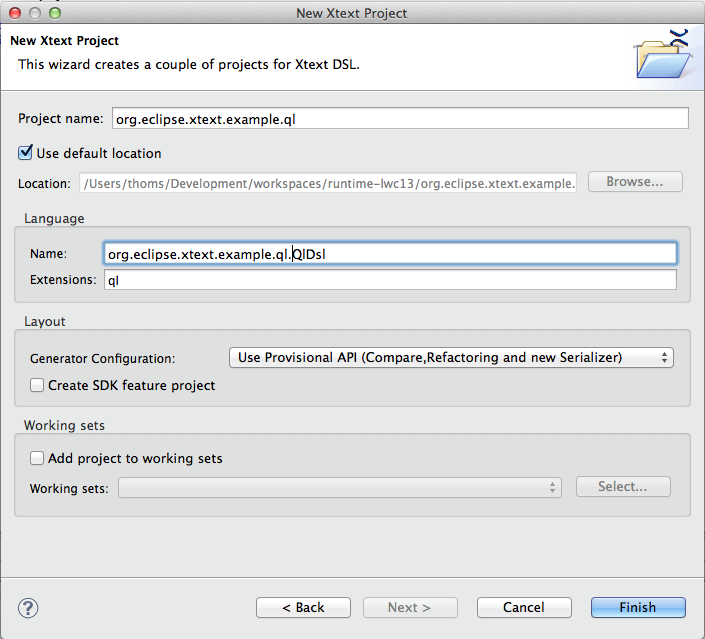
\includegraphics[width=17cm]{./images/chapter01/NewXtextProjectWizard.png}

On the project wizard page enter:
\begin{enumerate}
  \item Project name: \texttt{org.eclipse.xtext.example.ql}. Xtext will create
  multiple projects, which share this prefix. It is a convention to use
  a lowercase, dot-separated name.
  \item Language name: \texttt{org.eclipse.xtext.example.ql.QlDsl}. This is an
  identifier for the language, which must be unique and follows a Java
  full qualified Identifier name pattern.
  \item Language Extensions: \texttt{ql}. This will be the file extension for
  DSL files.
  \item Uncheck the option ``Create SDK feature project''. It would not harm to
  have that checked, it would just create an additional
  \href{http://www.vogella.com/articles/EclipseFeatureProject/article.html}{Feature
  Project}, which we do not handle in this tutorial any further.
\end{enumerate}

Now press ``Finish''. Xtext will generate you 3 projects into your workspace:

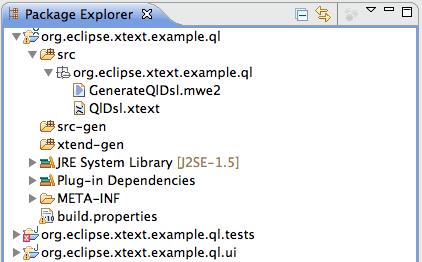
\includegraphics{./images/chapter01/WorkspaceAfterWizard.png}

\begin{itemize}
  \item \texttt{org.eclipse.xtext.example.ql}: This is the Runtime Project,
  which holds the language definition and any implementation which is not UI
  dependend. Most of the implementation details of this tutorial will be done in
  this project.
  \item \texttt{org.eclipse.xtext.example.ql.tests}: This project is intended to
  hold test code for the language. Tests are implemented with JUnit. Xtext will
  generate some infrastructure code required for tests into here. We won't deal
  testing of DSLs in this tutorial any further. You can close or remove this
  project if you want.
  \item \texttt{org.eclipse.xtext.example.ql.ui}: Xtext produces a language
  specific text editor. The editor is an Eclipse plugin. While the runtime part
  of the language could be used in any UI or even from command-line, the Editor
  is dependent on the Eclipse platform.
\end{itemize}

All projects are almost empty right now. Only the Runtime Project contains two
important files in the \texttt{/src} folder.
\begin{itemize}
  \item \texttt{GenerateQlDsl.mwe2}: This is a so-called ``MWE2 Workflow''. MWE
  is short for ``Modeling Workflow Engine'', which is a framework that is
  intended to define processes for code generation. This file defines the
  process to generate code for the DSL implementation.
  \item \texttt{QlDsl.xtext}: This is the file that contains the DSL language
  definition itself. It is called the \emph{Grammar} of the language.
\end{itemize}

